\part{微积分选讲}
\chapter{实数**}
\section{集合论概览}
\subsection{Russell悖论}
\clearpage
\subsection{集合的势}
\clearpage


\section{整数与有理数}
\subsection{整数的运算}
\clearpage
\subsection{有理数中的空隙}
\clearpage


\section{定义实数的若干种方法}
\subsection{Cantor的Cauchy列}
\clearpage
\subsection{Dedekind 分割}
\clearpage
\subsection{无穷小数法}
\clearpage
\subsection{实数的偏序性与基本定理}
\clearpage

\chapter{序列的极限**}
\section{从\texorpdfstring{\(\varepsilon-N\)}s开始}
\subsection{序列的极限定义}
\clearpage
\subsection{数列极限的性质}
\clearpage
\subsection{自然对数的底\texorpdfstring{$\e$}e与圆周率\texorpdfstring{$\pi$}e}
\clearpage

\section{级数的收敛}
\subsection{级数收敛的判别法}
\clearpage
\subsection{级数的运算和重排}
\clearpage

\chapter{函数极限与连续性**}
\section{函数极限的概念}
\subsection{函数极限的性质与概念}
\clearpage
\subsection{无穷大量与无穷小量}
\clearpage
\subsection{两个重要极限}
\clearpage
\section{连续函数}
\subsection{基本初等函数的连续性}
\clearpage
\subsection{有界闭区间上连续函数的性质}
\clearpage
\subsection{一致连续性}
\clearpage

\chapter{导数的初步认识}\label{导数的初步认识}
\section{导数的概念}
\subsection{从平均变化率到瞬时变化率}
\clearpage
\subsection{导数的几何意义}
\clearpage
\section{求导法则}
\subsection{基本初等函数的求导}
\clearpage
\subsection{导数的四则运算与复合函数的求导法则}
\clearpage
\subsection{反函数与其他坐标下的求导**}
\clearpage
\subsection{高阶导数*}
\clearpage

\section{用导数研究单调性与极值}
\subsection{导数与单调性的关系}
\clearpage
\subsection{导数与极值的关系}
\clearpage

%\subsection{三次函数}
\chapter{微分中值定理**}
\section{微分}
\subsection{微分的概念}
\clearpage
\subsection{三大中值定理}
\clearpage
\section{Taylor公式}
\subsection{不定式的极限}
\clearpage
\subsection{Taylor公式的推导和应用}
\clearpage

\subsection{求方程的近似解}
\clearpage
牛顿法


\chapter{导数的应用}
\section{用导数研究函数的例子}
\subsection{三次函数}


\begin{example}
    \(a > 0\)，函数 \(f(x) = x^4 + x^3 + ax + a^2\) 有且仅有两个不同的零点，求\(a\) 的取值范围。
\end{example}
\begin{jie}
    \


    \begin{way1}
        求导得\(f'(x)=4x^3+3x^2+a\). 常数项\(a\)可以看做对函数\(g(x)=4x^3+3x^2\)的平移. 因式分解得
        \(g(x)=x^2(4x+3)\), 由此绘制出图像
        \begin{figure}[H]

              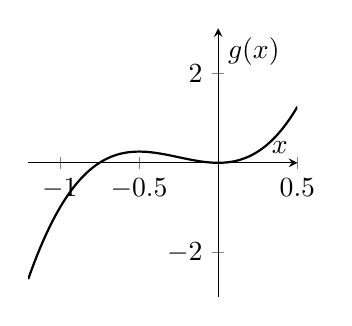
\begin{tikzpicture}
                \begin{axis}[
                    axis lines = middle, % 设置坐标轴为中间形式
                    xlabel = {$x$},     % x轴标签
                    ylabel = {$g(x)$},     % y轴标签
                    ymin = -3, ymax = 3, % y轴范围
                    xmin = -1.2, xmax = 0.5, % x轴范围
                    domain = -1.2:0.5,    % 函数的定义域
                    samples = 100,      % 采样点数量
                    width=5cm, height=5cm % 图像大小
                ]
                % 绘制函数图像
                \addplot [thick] {4*x^3 + 3*x^2};
                \end{axis}
               \end{tikzpicture}  
              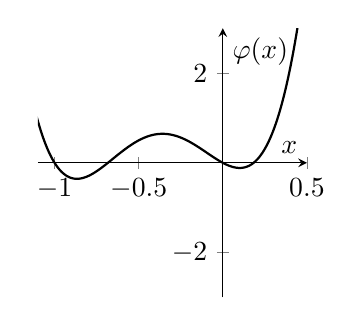
\begin{tikzpicture}
                \begin{axis}[
                    axis lines = middle, % 设置坐标轴为中间形式
                    xlabel = {$x$},     % x轴标签
                    ylabel = {$\varphi(x)$},     % y轴标签
                    ymin = -3, ymax = 3, % y轴范围
                    xmin = -1.1, xmax = 0.5, % x轴范围
                    domain = -1.2:0.5,    % 函数的定义域
                    samples = 1000,      % 采样点数量
                    width=5cm, height=5cm % 图像大小
                ]
                % 绘制函数图像
                \addplot [thick] {16*x^4 + 24*x^3+6*x^2-2*x^1};
                \end{axis}

            \end{tikzpicture}
            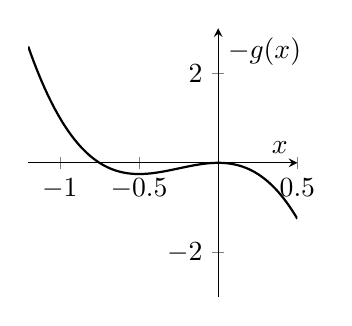
\begin{tikzpicture}
                \begin{axis}[
                    axis lines = middle, % 设置坐标轴为中间形式
                    xlabel = {$x$},     % x轴标签
                    ylabel = {$-g(x)$},     % y轴标签
                    ymin = -3, ymax = 3, % y轴范围
                    xmin = -1.2, xmax = 0.5, % x轴范围
                    domain = -1.2:0.5,    % 函数的定义域
                    samples = 100,      % 采样点数量
                    width=5cm, height=5cm % 图像大小
                ]
                % 绘制函数图像
                \addplot [thick] {-4*x^3 - 3*x^2};
                \end{axis}
               \end{tikzpicture}  
        \end{figure}
        由于\(a>0\), 从\(g(x)\)图像可见向上平移中不会为\(f'(x)\)增加更多零点了。即\(f'(x)\)在\(\mathbb{R}\)上有唯一的
        变号零点\(x_0\), 满足
        \begin{equation}
            4x_0^3+3x_0^2+a=0. 
        \end{equation}
        \(f(x)\)在\((-\infty,x_0)\)单调递减, 在\((x_0,+\infty)\)单调递增.因此只要\(f(x_0)<0\), 即可满足
        \(f(x)\)在\((-\infty,x_0)\)和\((x_0,+\infty)\)分别有唯一零点.

        在消去\(x_0\)和消去\(a\)的选择中, 这里选择了消\(a\), 带入\(a=-(4x_0^3+3x_0^2) \)
        \begin{align*}
            f(x)&=x^4_0+x^3_0+ax_0+a^2\\
                &=x^4_0+x^3_0+x_0(-4x_0^3-3x_0^2)+(-4x_0^3-3x_0^2)^2\\
                &=16x_0^6+24x_0^5+6x_0^4-2x_0^3\\
                &=2x_0^3(8x_0^3+12x_0^2+3x_0-1)\\
                &=2x_0^3(x_0+1)(8x_0^2+4x_0-1)
        \end{align*}
        设\(\varphi(x)=2x^3(x+1)(8x^2+4x-1)\), 其零点为\(-1,\frac{-1-\sqrt{3}}{4},0,\frac{-1+\sqrt{3}}{4}\).绘制出图像如所示,
        故使得\(f(x_0)<0\)的\(x_0\)取值范围是\((-1,\frac{-1-\sqrt{3}}{4})\cup(0,\frac{-1+\sqrt{3}}{4})\).
        
        别忘了\(x_0\)和\(a\)的关系\(-4x_0^3-3x_0^2=a\),我们需要把\(g(x)\)翻折一下. 由于\(a\)必须是正的,且\(\frac{-1-\sqrt{3}}{4}>-\frac{3}{4}\),
        在这个范围内,\(a\)的取值范围是\((0,1)\).
    \end{way1}
    \begin{way2}
        
    \end{way2}
\end{jie}

\clearpage
\subsection{三角函数}
\clearpage
\subsection{常见的函数不等式}
\begin{theorem}
    当 $x \geqslant 1$ 时，有 $\ln x \leqslant \frac{1}{2}\left(x - \frac{1}{x}\right)$；当 $0 < x \leqslant 1$ 时，有 $\ln x \geqslant \frac{1}{2}\left(x - \frac{1}{x}\right)$。当且仅当 $x = 1$ 时取等。
\end{theorem}
\begin{proof}
    考虑函数 $\varphi(x) = \ln x - \frac{1}{2}\left(x - \frac{1}{x}\right)$，其中 $x > 0$，计算得 $\varphi(1) = 0$，并且
\[
\varphi'(x) = \frac{1}{x} - \frac{1}{2} - \frac{1}{2x^2} = -\frac{(x-1)^2}{2x^2} \leqslant 0,
\]
从而可知 $\varphi(x)$ 在 $(0, +\infty)$ 内单调递减。因此，当 $x \geqslant 1$ 时，有 $\ln x \leqslant \frac{1}{2}\left(x - \frac{1}{x}\right)$；当 $0 < x \leqslant 1$ 时，有 $\ln x \geqslant \frac{1}{2}\left(x - \frac{1}{x}\right)$。
\end{proof}
\begin{theorem}
    当 $x \geqslant 1$ 时，有 $\ln x \geqslant \frac{2(x-1)}{x+1}$；当 $0 < x \leqslant 1$ 时，有 $\ln x \leqslant \frac{2(x-1)}{x+1}$。当且仅当 $x = 1$ 时取等。
\end{theorem}

\begin{proof}
    考虑函数 $\varphi(x) = \ln x - \frac{2(x-1)}{x+1}$，其中 $x > 0$，计算得 $\varphi(1) = 0$，并且
\[
\varphi'(x) = \frac{1}{x} - \frac{4}{(x+1)^2} = \frac{(x-1)^2}{x(x+1)^2} > 0,
\]
从而可知 $\varphi(x)$ 在 $(0, +\infty)$ 内单调递增。因此，当 $x \geqslant 1$ 时，有 $\ln x \geqslant \frac{2(x-1)}{x+1}$；当 $0 < x \leqslant 1$ 时，有 $\ln x \leqslant \frac{2(x-1)}{x+1}$。
\end{proof}

\tbox{
\[  \frac{2(x-1)}{x+1} \leqslant \ln x \leqslant \frac{1}{2}\left(x - \frac{1}{x}\right); (x\leq 1)\]
\[ \frac{1}{2}\left(x - \frac{1}{x}\right) \leqslant \ln x \leqslant \frac{2(x-1)}{x+1}.(0 < x \leqslant 1)\]

}
\begin{theorem}[对数均值不等式]
    设 $a$ 和 $b$ 是互异正数，则
\[
\sqrt{ab} < \frac{a-b}{\ln a - \ln b} < \frac{a+b}{2}.
\]
\end{theorem}
\begin{proof}
    不妨设 $a > b$。对于右边的不等式，整理得
\[
\ln a - \ln b = \ln \frac{a}{b} > \frac{2(a-b)}{a+b} = \frac{2\left(\frac{a}{b} - 1\right)}{\frac{a}{b} + 1},
\]
令 $t = \frac{a}{b} > 1$，则该不等式等价于 $\ln t > \frac{2(t-1)}{t+1}$，这是已经证明的结论。对于左边的不等式，整理得
\[
\ln a - \ln b = \ln \frac{a}{b} < \frac{a-b}{\sqrt{ab}} = \sqrt{\frac{a}{b}} - \sqrt{\frac{b}{a}},
\]
该不等式等价于 $\ln t < \sqrt{t} - \frac{1}{\sqrt{t}}$，这也是已经证明的结论。
\end{proof}

\clearpage

\section{恒成立问题}
\subsection{分类讨论}
\clearpage
\subsection{分离参数}
\clearpage
\subsection{必要性探路与端点效应}

\clearpage
\section{零点与极值点}
\subsection{隐零点问题}
\begin{example}[2012大纲全国卷]
    已知函数 $f(x) = \frac{1}{3}x^3 + x^2 + ax$.

\begin{enumerate}
    \item 讨论 $f(x)$ 的单调性；
    \item 设 $f(x)$ 有两个极值点 $x_1, x_2$，若过两点 $(x_1, f(x_1))$，$(x_2, f(x_2))$ 的直线 $l$ 与 $x$ 轴的交点在曲线 $y = f(x)$ 上，求 $a$ 的值。
\end{enumerate}
\end{example}

\begin{jie}
    \begin{enumerate}
        \item $f'(x) = x^2 + 2x + a, \Delta = 4 - 4a$.
        \begin{enumerate}
            \item 当 $\Delta = 4 - 4a \leq 0$，即 $a \geq 1$ 时，$f'(x) \geq 0, f(x)$ 在 $\mathbb{R}$ 上是增函数；
            \item 当 $a < 1$ 时，$f'(x) = 0$，有两个根 $x_1 = -1 - \sqrt{1-a}, x_2 = -1 + \sqrt{1-a}$。
            \begin{itemize}
                \item 当 $x \in (-\infty, -1 - \sqrt{1-a})$ 时 $f'(x) > 0, f(x)$ 是增函数；
                \item 当 $x \in (-1 - \sqrt{1-a}, -1 + \sqrt{1-a})$ 时 $f'(x) < 0, f(x)$ 是减函数；
                \item 当 $x \in (-1 + \sqrt{1-a}, +\infty)$ 时 $f'(x) > 0, f(x)$ 是增函数。
            \end{itemize}
        \end{enumerate}
        \item 由题设知，$x_1, x_2$ 为方程 $f'(x) = 0$ 的两个根，故由 (1) 有 $a < 1, x_1^2 = -2x_1 - a, x_2^2 = -2x_2 - a$。
        因此
        \begin{align*}
     f(x_1) &= \frac{1}{3}x_1^3 + x_1^2 + ax_1 = \frac{1}{3}x_1(-2x_1 - a) + x_1^2 + ax_1 \\
            &= \frac{1}{3}x_1^2 + \frac{2}{3}ax_1 = \frac{1}{3}(-2x_1 - a) + \frac{2}{3}ax_1 \\
            &= \frac{2}{3}(a-1)x_1 - \frac{a}{3}.
        \end{align*}
        同理，$f(x_2) = \dfrac{2}{3}(a-1)x_2 - \dfrac{a}{3}$。因此直线 $l$ 的方程为 $y = \dfrac{2}{3}(a-1)x - \dfrac{a}{3}$。
    
        设 $l$ 与 $x$ 轴的交点为 $(x_0, 0)$，将点代入 $l$ 得，$x_0 = \dfrac{a}{2(a-1)}$。因为点 $(x_0, 0)$ 在曲线 $y = f(x)$ 上，故
        \begin{align*}
          f(x_0) &= \frac{1}{3}\left[\frac{a}{2(a-1)}\right]^3 + \left[\frac{a}{2(a-1)}\right]^2 + \frac{a^2}{2(a-1)} \\
            &= \frac{a^2}{24(a-1)^3}(12a^2 - 17a + 6) = 0,
        \end{align*}
        解得 $a = 0$ 或 $a = \dfrac{2}{3}$ 或 $a = \dfrac{3}{4}$。
    \end{enumerate}
\qed
\end{jie}

\begin{example}[2012课标全国卷]
    设函数 $f(x) = e^x - ax - 2$.

\begin{enumerate}
    \item 求 $f(x)$ 的单调区间；
    \item 若 $a = 1, k$ 为整数，且当 $x > 0$ 时，$(x-k)f'(x) + x + 1 > 0$，求 $k$ 的最大值。
\end{enumerate}
\end{example}

\begin{jie}
\ 


\((1)\)$f(x)$ 的定义域为 $(-\infty, +\infty)$ $f'(x) = e^x - a$。
        \begin{itemize}
            \item 若 $a \leq 0$，则 $f'(x) > 0$，所以 $f(x)$ 在 $(-\infty, +\infty)$ 上单调递增。
            \item 若 $a > 0$，令 $f'(x) = e^x - a = 0$，得 $x = \ln a$。
            \begin{itemize}
                \item 当 $x \in (-\infty, \ln a)$ 时 $f'(x) < 0$；当 $x \in (\ln a, +\infty)$ 时 $f'(x) > 0$。所以 $f(x)$ 在 $(-\infty, \ln a)$ 上单调递减，在 $(\ln a, +\infty)$ 上单调递增。
            \end{itemize}
        \end{itemize}
        综上所述，
        \begin{itemize}
            \item 当 $a \leq 0$ 时 $f(x)$ 的增区间为 $(-\infty, +\infty)$；
            \item 当 $a > 0$ 时 $f(x)$ 的减区间为 $(-\infty, \ln a)$，增区间为 $(\ln a, +\infty)$。
        \end{itemize}

\((2)\)  
由于 $a = 1$，由 (1) 可得，$(x-k)f'(x) + x + 1 = (x-k)(e^x - 1) + x + 1$。
故当 $x > 0$ 时，$(x-k)f'(x) + x + 1 > 0$ 等价于 $$k < \frac{x+1}{e^x - 1} + x (x > 0)$$。

 令 $g(x) = \dfrac{x+1}{e^x - 1} + x$，则 $g'(x) = \dfrac{-xe^x - 1}{(e^x - 1)^2} + 1 = \dfrac{e^x(e^x - x - 2)}{(e^x - 1)^2}$。
 由于\(e^x>0\)恒成立，仅需要研究\(h(x) = e^x - x - 2\)的零点即可。
 
 由 (1) 知，函数 $h(x) = e^x - x - 2$ 在 $(0, +\infty)$ 上单调递增。
而 $h(1) = e - 3 < 0, h(2) = e^2 - 4 > 0$，所以 $h(x)$ 在 $(0, +\infty)$ 上存在唯一的零点，故 $g'(x)$ 在 $(0, +\infty)$ 上存在唯一的零点。
 设此零点为 $x_0$，则 $x_0 \in (1, 2)$。

当 $x \in (0, x_0)$ 时，$g'(x) < 0, g(x)$ 为减函数；当 $x \in (x_0, +\infty)$ 时，$g'(x) > 0, g(x)$ 为增函数。
 所以 $g(x)$ 在 $(0, +\infty)$ 上的最小值为 $g(x_0)$。
 又由 $g'(x_0) = 0$，可得 $e^{x_0} = x_0 + 2$，所以 $g(x_0) = x_0 + 1 \in (2, 3)$。
由于等价于 $k < g(x_0)$，故整数 $k$ 的最大值为 2。
\qed
\end{jie}
\begin{example}[2017年II卷理]
    已知函数 $f(x) = x^2 - x - x\ln x$，证明：$f(x)$ 存在唯一的极大值点 $x_0$，且 $e^{-2} < f(x_0) < 2^{-2}$。
\end{example}
\begin{jie}
    首先，计算得
    \[
    f'(x) = 2x - 2 - \ln x, \quad f''(x) = \frac{2x - 1}{x},
    \]
    因此 $f'(x)$ 在 $\left(0, \frac{1}{2}\right)$ 内单调递减，在 $\left(\frac{1}{2}, +\infty\right)$ 内单调递增。又
    \[
    f'\left(\frac{1}{e^2}\right) = \frac{2}{e^2} > 0, \quad f'\left(\frac{1}{2}\right) = \ln 2 - 1 < 0, \quad f'(1) = 0,
    \]
    因此存在 $x_0 \in \left(\frac{1}{e^2}, \frac{1}{2}\right)$，使得 $f'(x_0) = 0$。
    
    在上面我们得到了 $f'(x_0) = 2x_0 - 2 - \ln x_0 = 0$。$f(x)$ 在 $(0, x_0)$ 内单调递增，在 $(x_0, 1)$ 内单调递减，在 $(1, +\infty)$ 内单调递增，因此 $x = x_0$ 是 $f(x)$ 的极大值点。一方面，有
    \[
    f(x_0) = x_0^2 - x_0 - x_0\ln x_0 = x_0^2 - x_0 - x_0(2x_0 - 2) = x_0(1 - x_0) < \frac{1}{4} = 2^{-2};
    \]
    另一方面，根据 $x_0$ 是极大值点得
    \[
    f(x_0) > f\left(\frac{1}{e}\right) = e^{-2},
    \]
    因此 $f(x)$ 存在唯一的极大值点 $x_0$，且 $e^{-2} < f(x_0) < 2^{-2}$。








    \qed
\end{jie}
\begin{exercise}[2019年II卷文数]
    已知函数 $f(x) = (x-1)\ln x - x - 1$。证明：
\begin{enumerate}
    \item $f(x)$ 存在唯一的极值点；
    \item $f(x) = 0$ 有且仅有两个实根，且两个实根互为倒数。
\end{enumerate}

\end{exercise}

\begin{proof}
\ 

\((1)\)$f(x)$ 的定义域为 $(0, +\infty)$，计算得 $f'(x) = \ln x - \dfrac{1}{x}$，由 $\ln x$ 与 $-\dfrac{1}{x}$ 在 $(0, +\infty)$ 内单调递增知 $f'(x)$ 在 $(0, +\infty)$内单调递增，计算得
        \[ f'(1) = -1 < 0,  \quad f'(e) = 1 - \frac{1}{e} > 0. \]
     故根据零点定理知，存在 $x_0 \in (1, e)$，使得 $f'(x_0) = 0$，$f(x)$ 在 $(0, x_0)$ 内单调递减，在 $(x_0, +\infty)$ 内单调递增，$x = x_0$ 是 $f(x)$
     的极小值点。

\((2)\)计算得 $f(e) = -2 < 0$，$f(e^2) = e^2 - 3 > 0$，故根据零点定理知，存在 $x_1 \in (e, e^2)$，使得 $f(x_1) = 0$
    。注意到此时
        \[
        f
    \left(\frac{1}{x}\right) = -\left(\frac{1}{x} - 1\right)\ln x - \frac{1}{x} - 1 = \frac{(x-1)\ln x - x - 1}{x} = \frac
    {f(x)}{x},
        \]
        因此当且仅当 
    $f\left(\frac{1}{x}\right) = 0$ 时 $f(x) = 0$，从而 $x_2 = \frac{1}{x_1}$ 也是 $f(x)$ 的零点，根据单调性知 $f(x)$ 有且仅有两个零点 $x_1$ 和 $x_2$
    。

    \qed
\end{proof}

\begin{example}[2022年新高考I卷]
    已知函数\(f(x)=e^x-ax\)和\(g(x)=ax-\ln x\)有相同的最小值.
    \begin{enumerate}
        \item 求\(a\)的值；
        \item 证明：存在直线 $y = b$，其与两条曲线 $y = f(x)$ 和 $y = g(x)$ 共有三个不同的交点，并且从左到右的三个交点的横坐标成等差数列。
    \end{enumerate}
\end{example}
\begin{jie}
\  

\((1)\)$f(x)$ 的定义域为 $\mathbb{R}$，$f'(x) = e^x - a$，由 $f(x)$ 有最小值得 $a > 0$，且 $f(x)_{\min} = f(\ln a) = a - a\ln a$；

同时\(g(x)\)的定义域为\((0,+\infty)\)，$g'(x) = \dfrac{ax - 1}{x}$，
从而 $g(x)_{\min} = g\left(\dfrac{1}{a}\right) = 1 + \ln a$。

由\(f_{\min}(x)=g_{\min}(x)\)得
$$ \ln a - \dfrac{a-1}{a+1} = 0$$。
            
        令 $h(a) = \ln a - \dfrac{a-1}{a+1}$，其中 $a > 0$，计算得
        \[ h'(a) = \frac{1}{a} - \frac{2}{(a+1)^2} = \frac{a^2 + 1}{a(a+1)^2} > 0, \]
        因此 $h(a)$ 在 $(0, +\infty)$ 内单调递增，注意到 $h(1) = 0$，于是 $h(a)$ 的唯一零点是 $a = 1$。
        
\((2)\)不妨设 $x_1 < 0 < x_2 < 1 < x_3$ ，此时
    \[e^{x_1} - x_1 = e^{x_2} - x_2 = x_2 - \ln x_2 = x_3 - \ln x_3. \]

    首先，注意到
        \[f(x_1) = e^{x_1} - x_1 = g(x_2) = x_2 - \ln x_2 = e^{\ln x_2} - \ln x_2 = f(\ln x_2),\]
    其中 $x_1 < 0, \ln x_2 < 0$，根据 $f(x)$ 在 $(-\infty, 0)$ 内单调递减，
    知 $x_1 = \ln x_2$，即 $x_2 = e^{x_1}$。
    
    接下来，注意到
    \[f(x_2) = e^{x_2} - x_2 = g(x_3) = x_3 - \ln x_3 = e^{\ln x_3} - \ln x_3 = f(\ln x_3),  \]
    其中 $x_2 > 0, \ln x_3 > 0$，根据 $f(x)$ 在 $(0, +\infty)$ 内单调递增，知 $x_2 = \ln x_3$，即 $x_3 = e^{x_2}$。最后，计算得
     \[x_1 + x_3 = \ln x_2 + e^{x_2} = 2x_2,\]
    从而 $x_1, x_2, x_3$ 成等差数列。
    \qed
\end{jie}



含参的处理：

\begin{example}[2009 全国 II 理 ]
    设 $f(x) = x^2 + a \ln(1 + x)$ 有两个极值点 $x_1, x_2$，且 $x_1 < x_2$。
\begin{enumerate}
    \item 求实数 $a$ 的取值范围，并讨论 $f(x)$ 的单调性；
    \item 证明：$f(x_2) > \dfrac{1 - 2\ln 2}{4}$。
\end{enumerate}
\end{example}

\begin{jie}
    \                  

    \((1)\)原问题等价于 $f'(x) = \dfrac{2x^2 + 2x + a}{1 + x}$ 在 $(-1, +\infty)$ 上有两个零点 $x_1, x_2$，即 $h(x) = 2x^2 + 2x + a$ 在 $(-1, +\infty)$ 上有两个零点 $x_1, x_2$，如图 5-22 所示，则原问题等价于
    \[
    \begin{cases}
        \Delta = 4 - 8a > 0 \\
        h(-1) > 0
    \end{cases}
    \]
    解得 $0 < a < \dfrac{1}{2}$，且此时 $f(x)$ 在 $(-1, x_1)$ 上单调递增，在 $(x_1, x_2)$ 上单调递减，在 $(x_2, +\infty)$ 上单调递增。

    \((2)\)原问题等价于证明
    \[
    \begin{cases}
        2x_2^2 + 2x_2 + a = 0 \\
        f(x_2) = x_2^2 + a \ln(1 + x_2) > \dfrac{1 - 2\ln 2}{4}
    \end{cases}
    \]
    在 $a \in \left(0, \frac{1}{2}\right)$上恒成立。由第一个方程可得
    \[a = -2x_2^2 - 2x_2 \]
    代入式 (5.6.1) 的第二个方程可得
    \[f(x_2) = x_2^2 - 2(x_2 + x_2^2) \ln(1 + x_2) > \frac{1 - 2\ln 2}{4} \]
    显然不等式并不是对所有的 $x_2 \in (-1, +\infty)$ 都成立（$x_2$ 趋于 $+\infty$ 会产生矛盾）。
    考虑\(h(0)=a\in(0,\dfrac{1}{2})\)，可知 $x_2 \in \left(-\dfrac{1}{2}, 0\right)$。

    故原问题等价于证明 $$g(t) = t^2 - 2(t + t^2) \ln(1 + t) > \frac{1 - 2\ln 2}{4}$$
    在 $\left(-\dfrac{1}{2}, 0\right)$上恒成立，求导得
    \[g'(t) = -2(1 + 2t) \ln(1 + t) > 0, \]
    即 $g(t)$ 在 $\left(-\dfrac{1}{2}, 0\right)$ 上单调递增。
    故 $g(t) > g\left(-\dfrac{1}{2}\right) = \dfrac{1}{4} - \dfrac{2\ln 2}{4}$，这就证明了 $f(x_2) > \dfrac{1 - 2\ln 2}{4}$。

    \qed
\end{jie}

\begin{example}[2021年天津]
    已知 $a > 0$，函数 $f(x) = ax - xe^x$。
\begin{enumerate}
    \item 证明 $f(x)$ 存在唯一的极值点；
    \item 若存在 $a$，使得 $f(x) \leqslant a + b$ 对任意 $x \in \mathbb{R}$ 成立，求实数 $b$ 的取值范围。
\end{enumerate}
\end{example}
\begin{jie}
    \ 

    \((1)\)计算得
    \[
    f'(x) = a - (x + 1)e^x, \quad f''(x) = -(x + 2)e^x,
    \]
    因此 $f'(x)$ 在 $(-\infty, -2)$ 内单调递增，在 $(-2, +\infty)$ 内单调递减，
    当 $x \to -\infty$ 时，$f'(x) \to a > 0$，且 $f'(-1) = a > 0$，
    当 $x \to +\infty$ 时，$f'(x) \to -\infty$，
    因此存在 $x_0 \in (-1, +\infty)$，使得 $f'(x_0) = 0$，
    $x = x_0$ 是 $f(x)$ 的极值点，且满足 $(x_0 + 1)e^{x_0} = a$。


    \((2)\)
    首先固定 $a$，则由 $(x_0 + 1)e^{x_0} = a$ 知 $x_0$ 也固定。令 $g(x) = f(x) - a$，则 $g'(x) = f'(x)$，$g(x)$ 在 $(-\infty, x_0)$ 内单调递增，在 $(x_0, +\infty)$ 内单调递减，从而
    \[g(x)_{\max} = g(x_0) = ax_0 - x_0e^{x_0} - a = (x_0^2 - x_0 - 1)e^{x_0} \leqslant b.\]
    令 $\varphi(x) = (x^2 - x - 1)e^x$，其中 $x > -1$，计算得
    \[\varphi'(x) = (x^2 + x - 2)e^x = (x - 1)(x + 2)e^x,\]
    因此 $\varphi(x)$ 在 $(-1, 1)$ 内单调递减，在 $(1, +\infty)$ 内单调递增，
    $\varphi(x)_{\max} = \varphi(1) = -e$，因此实数 $b$ 的取值范围是 $[-e, +\infty)$。

    \qed
\end{jie}

















\begin{example}
    求证：\(e^x-\ln x >2\).
\end{example}




















\begin{example}
    求证：\(e^x-\ln x >2.3\);（参考值：\(\sqrt{\e}=1.649,\ln 2=0.693,\dfrac{4}{3}\sqrt{3}=2.3094\)）.
\end{example}

\begin{proof}
    设 $f(x) = e^x - \ln x$，定义域 $x \in (0, +\infty)$，则 $f'(x) = e^x - \frac{1}{x}$ 在 $x \in (0, +\infty)$ 上为增函数。

又 $f'\left(\frac{1}{2}\right) = \sqrt{e} - 2 < 0$，$f'(1) = e - 1 > 0$，所以存在唯一 $x_0 \in \left(\frac{1}{2}, 1\right)$，使得 $f'(x_0) = 0$。

所以当 $x \in (0, x_0)$ 时 $f'(x) < 0$，$f(x)$ 在 $x \in (0, x_0)$ 上单调递减；

当 $x \in (x_0, +\infty)$ 时 $f'(x) > 0$，$f(x)$ 在 $x \in (x_0, +\infty)$ 上单调递增。

所以 $f(x)_{\min} = f(x_0) = e^{x_0} - \ln x_0$，

又 $f'(x_0) = 0$，即 $e^{x_0} = \frac{1}{x_0}$，两边取对数得 $x_0 = -\ln x_0$，都代入得

\[ f(x)_{\min} = f(x_0) = \frac{1}{x_0} + x_0 \]，在 $x_0 \in \left(\frac{1}{2}, 1\right)$ 上为减函数，

所以 $f(x_0) > f(1) = 2$，不满足题意。

又 $f\left(\frac{1}{2}\right) = \sqrt{e} + \ln 2 > 2.3$，说明 $x_0$ 范围估值不够精确，需进一步缩小范围。

又 $x_0 = -\ln x_0$ 说明 $x_0$ 是一个不精确计算出的值，

而当 $x \in (0, 1)$ 时，有 $\ln x > \frac{1}{2}(x - \frac{1}{x})$，于是

\[ x = -\ln x < -\frac{1}{2}(x - \frac{1}{x}) \]，解得 $x < \frac{1}{\sqrt{3}}$，

所以进一步确定 $x_0 \in \left(\dfrac{1}{2}, \dfrac{1}{\sqrt{3}}\right)$，有 $f(x_0) > f\left(\dfrac{1}{\sqrt{3}}\right) = \sqrt{3} + \dfrac{1}{\sqrt{3}} = \dfrac{4\sqrt{3}}{3} > 2.3$。

综上所述，$e^x - \ln x > 2.3$。
\qed
\end{proof}

\begin{definition}
    设函数\(f(x)=x\e ^x,x\in\mathbb{R}\)，则记\(W(x)\)为\(f(x)(x\geq -1)\)的反函数，\(W_{-1}(x)\)为\(f(x)(x\leq -1)\)
    的反函数。函数\(W(x)\)和\(W_{-1}(x)\)称为Lambert函数。(Lambert W Functionf)
\end{definition}
















\clearpage
\subsection{多变量的基本处理}
\clearpage
\subsection{极值点偏移}

\begin{example}[2010年天津理]
    已知函数 $f(x) = \dfrac{x}{e^x}$，如果 $x_1 \neq x_2$，且 $f(x_1) = f(x_2)$，证明：$x_1 + x_2 > 2$。
\end{example}

\begin{proof}
    $f'(x) = (1-x)e^{-x}$，故 $f(x)$ 在 $(-\infty, 1)$ 上递增，在 $(1, +\infty)$ 上递减。不妨设 $x_1 < x_2$，由 $f(x_1) = f(x_2)$ 可得 $x_1 < 1$，$x_2 > 1$，由 $f(x_1) = f(x_2)$ 可得
    \[
    x_1 + x_2 > 2 \Rightarrow x_1 > 2 - x_2 \Rightarrow f(x_1) > f(2 - x_2) \Rightarrow f(x_2) > f(2 - x_2)
    \]
    即只需证 $g(x) = f(x) - f(2-x) = xe^{-x} - (2-x)e^{x-2} > 0$ 在 $(1, +\infty)$ 上成立。求导可得 $g'(x) = (x-1)(e^{x-2} - e^{-x})$。因为 $h(x) = e^{x-2} - e^{-x}$ 在 $(1, +\infty)$ 上递增，所以 $h(x) > h(1) = 0$，因此 $g'(x) = (x-1)h(x) > 0$ 在 $(1, +\infty)$ 上恒成立。因此 $g(x)$ 在 $(1, +\infty)$ 上递增，故 $g(x) > g(1) = f(1) - f(1) = 0$，即 $f(x) > f(2-x)$，因此 $f(x_2) > f(2-x_2)$。故
    \[
    f(x_2) > f(2 - x_2) \Rightarrow f(x_1) > f(2 - x_2) \Rightarrow x_1 + x_2 > 2
    \]
    
\end{proof}


\begin{example}
    若 $m > 1$ 且 $x_1, x_2$ 为 $g(x) = \ln(x+m) - x$ 的两个零点，证明：$x_1 + x_2 < 0$。
\end{example}
\begin{analyse}
    \(0\)不是原函数的极值点。考虑分参。
\end{analyse}
\begin{proof}
    因为 $x_1, x_2$ 为 $g(x)$ 的两个零点，所以 $x_1, x_2$ 为 $h(x) = e^x - x - m$ 的两个零点。求导可得 $h'(x) = e^x - 1$，故 $h(x)$ 在 $(0, +\infty)$ 上单调递增，在 $(-m, 0)$ 上单调递减。不妨设 $x_1 < x_2$，由 $h(x_1) = h(x_2)$ 可知 $x_1 < 0 < x_2$
，则
\[
x_1 + x_2 < 0 
\Leftrightarrow x_1 < -x_2 \Leftrightarrow h(x_1) > h(-x_2) \Leftrightarrow
 h(x_2) > h(-x_2)
\]
然后构造函数 
$F(x) = h(x) - h(-x)$，因为 $h(x)$ 的定义域为 $(-m, +\infty)$，所以 $h(-x)$ 的定义域为 $(-\infty, m)$，因此 $F(x)$ 的定义域为 $(-m, m)$。又因为我们关心的是 $F(x_2)$ 的符号且 $x_2 > 0$，所以只需证明函数 $F(x) > 0$ 在 $(0, m)$ 上成立即可。因为 $F(0) = 0$，所以只需证明 $F(x)$ 在 $(0, m)$
 上单调递增即可。

因为 
$F(x) = e^x - \frac{1}{e^x} - 2x$，则求导可得 $F'(x) = e^x + \frac{1}{e^x} - 2$，当 $x \in (0, m)$ 时，$F'(x) > 0$，即 $F(x)$ 在 $(0, m)$ 上单调递增，故 $x_1 + x_2 < 0$
 得证。

\end{proof}

\begin{example}
    已知函数 $f(x) = \frac{1 + \ln x}{x}$，若 $f(x) = m$ 有两个不同实根 $x_1, x_2$，求证：$\frac{1}{x_1} + \frac{1}{x_2} > 2$。
\end{example}

\begin{proof}
    所证结论 $\frac{1}{x_1} + \frac{1}{x_2} > 2$ 并不是常见类型，怎么办？把它化成常规类型，通常情况下都是换元法：令 $t_1 = \frac{1}{x_1}, t_2 = \frac{1}{x_2}$，即证明 $t_1 + t_2 > 2$。接下来需要找出 $t_1, t_2$ 所满足的方程。

由 $f(x_1) = f(x_2) = m$，可知 $1 + \ln x_1 = mx_1$，$1 + \ln x_2 = mx_2$，可得 $t_1 - t_1 \ln t_1 = t_2 - t_2 \ln t_2$。令 $g(t) = t - t \ln t$，则 $g(t_1) = g(t_2)$。

则原问题等价于“已知函数 $g(t) = t - t \ln t$，且 $t_1, t_2$ 满足 $g(t_1) = g(t_2)$，证明：$t_1 + t_2 > 2$”。求导可得 $g'(t) = -\ln t$，则 $g(t)$ 在 $(1, +\infty)$ 上单调递减，在 $(0, 1)$ 上单调递增，因为 $g(t_1) = g(t_2)$，不妨设 $0 < t_1 < 1 < t_2$，则
\[
t_1 + t_2 > 2 \Leftrightarrow t_1 > 2 - t_2 \Leftrightarrow g(t_1) > g(2 - t_2) \Leftrightarrow g(t_2) > g(2 - t_2)
\]
求导可得然后构造辅助函数 $F(t) = g(t) - g(2-t)$，因为 $g(t)$ 的定义域为 $(0, +\infty)$，所以 $g(2-t)$ 的定义域为 $(-\infty, 2)$，因此 $F(t)$ 的定义域为 $(0, 2)$。又因为我们关心的是 $F(t_2)$ 的符号且 $t_2 > 1$，所以只需证明函数 $F(t) > 0$ 在 $(1, 2)$ 上成立即可。因为 $F(1) = 0$，所以只需证明 $F(t)$ 在 $(1, 2)$ 上单调递增即可。

令 $F(t) = g(t) - g(2-t)$，$t \in (1, 2)$，则 $F'(t) = -\ln(2-t) - \ln t = -\ln t(2-t) > -\ln\left(\frac{t+2-t}{2}\right)^2 = 0$，即 $F(t)$ 在 $(1, 2)$ 上单调递增。故 $\frac{1}{x_1} + \frac{1}{x_2} > 2$ 得证。
\end{proof}
\begin{example}
    若 $f(x) = x^2 \ln x - m$ 有两个不同零点 $x_1, x_2$，求证：$x_1^2 + x_2^2 > \frac{2}{e}$。
\end{example}
\begin{proof}
    令 $t_1 = x_1^2, t_2 = x_2^2$，由 $f(x_1) = f(x_2)$，可得 $x_1^2 \ln x_1 = x_2^2 \ln x_2$，即 $t_1 \ln t_1 = t_2 \ln t_2$，记函数 $h(t) = t \ln t$，即证 $t_1 + t_2 > \frac{2}{e}$。求导可得 $h'(t) = 1 + \ln t$，当 $x \in \left(0, e^{-1}\right)$ 时，函数 $h(x)$ 单调递减，当 $x \in \left(e^{-1}, +\infty\right)$ 单调递增。不妨设 $t_1 < t_2$，因为 $h(t_1) = h(t_2)$，所以 $t_1 < \frac{1}{e} < t_2$，则
\[
t_1 + t_2 > \frac{2}{e} \Leftrightarrow t_1 > \frac{2}{e} - t_2 \Leftrightarrow h(t_1) > h\left(\frac{2}{e} - t_2\right) \Leftrightarrow h(t_2) > h\left(\frac{2}{e} - t_2\right)
\]
令 $F(t) = h(t) - h\left(2e^{-1} - t\right)$，因为 $h(t)$ 的定义域为 $(0, +\infty)$，所以 $h\left(2e^{-1} - t\right)$ 的定义域为 $(-\infty, 2e^{-1})$。$F(t) = h(t) - h\left(2e^{-1} - t\right)$，因为 $h(t)$ 的定义域为 $(0, 2e^{-1})$ 上的符号，因此只考虑 $F(t)$ 在 $(e^{-1}, 2e^{-1})$ 上的符号即可。求导可得 $F'(t) = 2 + \ln\left(t(2e^{-1} - t)\right) < 0$，故 $F(t)$ 在 $(e^{-1}, 2e^{-1})$ 上递减，即 $F(t_2) < F(e^{-1}) = 0$，故 $x_1^2 + x_2^2 > \frac{2}{e}$ 得证。
\end{proof}
\begin{example}
    已知函数 $f(x) = \ln x - ax$，若函数 $f(x)$ 有两个零点 $x_1, x_2$，证明：$x_1 x_2 > e^2$。
\end{example}

\begin{proof}
    显然 $x = e$ 不为 $f(x)$ 的极值点，因此先通过分离变量可得 $a = \frac{\ln x}{x}$。令 $g(x) = \frac{\ln x}{x}$。求导可得 $g'(x) = \frac{1 - \ln x}{x^2}$，则 $g(x)$ 在 $(0, e)$ 上递增，在 $(e, +\infty)$ 上递减。不妨设 $0 < x_1 < x_2$ 且 $g(x_1) = g(x_2)$，则 $0 < x_1 < e < x_2$，故
\[
x_1 x_2 > e^2 \Leftrightarrow x_1 > \frac{e^2}{x_2} \Leftrightarrow g(x_1) > g\left(\frac{e^2}{x_2}\right) \Leftrightarrow g(x_2) > g\left(\frac{e^2}{x_2}\right)
\]
令 $h(x) = g(x) - g\left(\frac{e^2}{x}\right)$，因为 $g(x)$ 的定义域为 $(0, +\infty)$，所以 $g\left(\frac{e^2}{x}\right)$ 的定义域为 $(0, +\infty)$，故 $h(x)$ 的定义域为 $(0, +\infty)$。又因为我们关心的是 $h(x_2)$ 的符号，因此我们只需研究 $h(x)$ 在 $(e, +\infty)$ 上的符号即可。求导可得 $h'(x) = (1 - \ln x)\left(\frac{1}{x^2} - \frac{1}{e^2}\right) > 0$ 在 $(e, +\infty)$ 上恒成立。故 $h(x_2) > h(e) = 0$，即 $x_1 x_2 > e^2$ 得证。
\end{proof}

\begin{example}[2021年新高考I卷]
    已知函数 $f(x) = x(1 - \ln x)$。

\begin{enumerate}
    \item 讨论 $f(x)$ 的单调性；
    \item 设 $a, b$ 为两个不相等的正实数，且 $b \ln a - a \ln b = a - b$，证明：$2 < \frac{1}{a} + \frac{1}{b} < e$。
\end{enumerate}

\end{example}
\begin{jie}
    
\end{jie}


极值点被放缩过

\begin{example}
    已知函数 $f(x) = \frac{1}{2}x^2 + (1-a)x - a\ln x, a \in \mathbb{R}$.
若 $f(x)$ 存在两个不同零点 $x_1, x_2$，求证：$x_1 + x_2 > 2$。
\end{example}
\begin{jie}
    \begin{align*}
        f'(x) &= x + 1 - a - \frac{a}{x} = (x + 1) - \frac{a(x + 1)}{x} \\
        &= (x + 1)\left(1 - \frac{a}{x}\right) \\
        \text{if } a \leqslant 0, & \ f'(x) > 0, \text{ wrong} \Rightarrow a > 0 \\
        x \in (0, a), & \ f'(x) < 0, x \in (a, +\infty), f'(x) > 0 \\
        f'(x) = 0 & \Rightarrow x = a
        \end{align*}
        
        我们发现，这里的极值点是 $a$，如果是标准的偏移，应该是证明 $x_1 + x_2 > 2a$。但题目却嚷证明 $x_1 + x_2 > 2$，我们一时难以理解。
        \begin{align*}
            f(x)_{\min} &= f(a) = \frac{a^2}{2} + (1-a)a - a\ln a < 0 \\
            \Rightarrow \frac{a}{2} + 1 - a - \ln a &= 1 - \frac{a}{2} - \ln a < 0 \\
            h(a) &= 1 - \frac{a}{2} - \ln a, h(1) = 1 - \frac{1}{2} = \frac{1}{2} > 0 \\
            \Rightarrow a &> 1
            \end{align*}
            
            要使 $f(x)$ 有两个不同零点，则 $f(x)$ 的最小值（极小值）必小于零，因此，我们要解出这个关于 $a$ 的不等式的解集。然而，我们发现这个不等式是超越的。
            
            虽然不能解出 $a$ 的具体范围，但我们可以得到一个必要条件，即 $a > 1$，所以，要证明原问题的 $x_1 + x_2 > 2$，我们只需要证明 $x_1 + x_2 > 2a$ 即可。而 $2a$ 刚好是我们 2 倍的极值点，所以，我们已经把问题转化成了极值点偏移的标准形式。
            
            \begin{align*}
            f'(x) &= x + 1 - a - \frac{a}{x} = (x + 1) - \frac{a(x + 1)}{x} \\
            &= (x + 1)\left(1 - \frac{a}{x}\right) \\
            \text{if } a \leqslant 0, & \ f'(x) > 0, \text{ wrong} \Rightarrow a > 0 \\
            x \in (0, a), & \ f'(x) < 0, x \in (a, +\infty), f'(x) > 0 \\
            f'(x) = 0 & \Rightarrow x = a \\
            f(x)_{\min} &= f(a) = \frac{a^2}{2} + (1-a)a - a\ln a < 0 \\
            \Rightarrow \frac{a}{2} + 1 - a - \ln a &= 1 - \frac{a}{2} - \ln a < 0 \\
            h(a) &= 1 - \frac{a}{2} - \ln a, h(1) = 1 - \frac{1}{2} = \frac{1}{2} > 0 \\
            \Rightarrow a &> 1, 0 < x_1 < a < x_2, 2a - x_2 < a \\
            x_1 + x_2 > 2a &\Leftarrow x_1 > 2a - x_2 \Leftarrow f(x_1) < f(2a - x_2) \\
            \Leftrightarrow f(x_2) - f(2a - x_2) &< 0, \\
            F(x) &= f(x) - f(2a - x) = 2x - a\ln x + a\ln(2a - x) - 2a \\
            F'(x) &= 2 - \frac{a}{x} - \frac{a}{2a - x} = -\frac{2(x - a)^2}{x(2a - x)} \leqslant 0 \\
            \therefore F(x) &< F(a) = 0 \Rightarrow x_1 + x_2 > 2a > 2
            \end{align*}
            
            \qed
\end{jie}





\clearpage
\subsection{零点差}
\clearpage

\section{复杂函数的处理手段}
\subsection{凹凸反转}
\clearpage
\subsection{相同结构的函数——“同构”}

\begin{example}[2022年武汉二调]
    已知函数 $f(x) = a|\ln x| + x + \dfrac{1}{x}, g(x) = e^x + e^{-x} - a|\ln(ax)| - \dfrac{1}{ax}$，其中 $a > 0$.
        (1) 当 $a = 1$ 时，求 $\frac{f'\left(\frac{1}{e}\right)}{f'(e)}$ 的值；
        (2) 讨论 $g(x)$ 的零点个数。
\end{example}
\begin{jie}
\ 

$(1)$当 $a=1$ 时，$f(x) = |\ln x| + x + \frac{1}{x}$。

当 $0 < x < 1$ 时，$f(x) = -\ln x + x + \frac{1}{x}$，$f'(x) = -\frac{1}{x} + 1 - \frac{1}{x^2}$，$f'\left(\frac{1}{e}\right) = -e + 1 - e^2$。

当 $x > 1$ 时，$f(x) = \ln x + x + \frac{1}{x}$，$f'(x) = \frac{1}{x} + 1 - \frac{1}{x^2}$，$f'(e) = \frac{1}{e} + 1 - \frac{1}{e^2} = \frac{e^2 + e - 1}{e^2}$。

\[
\frac{f'\left(\frac{1}{e}\right)}{f'(e)} = -e^2.
\]


$(2) $令 $g(x) = 0$，有 $e^x + e^{-x} = a|\ln(ax)| + \frac{1}{ax}$。
    
则 $ax + e^x + e^{-x} = a|\ln(ax)| + ax + \frac{1}{ax}$，即 $a|\ln e^x| + e^x + e^{-x} = a|\ln(ax)| + ax + \frac{1}{ax}$。
所以 $f(e^x) = f(ax)$。

关注\(f(x)\)的单调性：
    \[
    \begin{aligned}
        &0 < x < 1 , f'(x) = -\frac{a}{x} + 1 - \frac{1}{x^2} = -\frac{a}{x} - \frac{1-x^2}{x^2} < 0; \\
        &x > 1 ,f'(x) = \frac{a}{x} + 1 - \frac{1}{x^2} = \frac{a}{x} + \frac{x^2-1}{x^2} > 0;
    \end{aligned}
    \]
所以，$f(x)$ 在 $(0,1)$ 上递减；在 $(1,+\infty)$ 上递增。
    
    又因为 $f(x) = f\left(\frac{1}{x}\right)$，所以 $f(e^x) = f(ax)$，当且仅当 $e^x = ax$ 或 $e^x = \frac{1}{ax}$。
    又 $e^x > 1$，故 $e^x = ax$ 和 $e^x = \frac{1}{ax}$ 不可能同时成立。
    所以 $g(x)$ 的零点个数是两个函数 $s(x) = e^x - ax$ 和 $t(x) = xe^x - \frac{1}{a}$ 的零点个数之和，其中 $x > 0$。
    
    $s'(x) = e^x - a$，$0 < a \leq 1$ 时，$s'(x) > 0$，$s(x)$ 递增，$s(x) > s(0) = 1$，$s(x)$ 无零点。
    
    $a > 1$ 时，令 $s'(x) = 0$，得 $x = \ln a$，故 $s(x)$ 在 $(0, \ln a)$ 上递减；在 $(\ln a, +\infty)$ 上递增。
    
    当 $1 < a < e$ 时，$s(\ln a) = a(1 - \ln a) > 0$，此时 $s(x)$ 无零点。
    
    当 $a = e$ 时，$s(\ln a) = 0$，此时 $s(x)$ 有一个零点。
    
    当 $a > e$ 时，$s(\ln a) = a(1 - \ln a) < 0$，$s\left(\frac{1}{a}\right) = e^{\frac{1}{a}} - 1 > 0$，$s(2\ln a) = a^2 - 2a\ln a = a(a - 2\ln a)$。
    
    令 $h(a) = a - 2\ln a \ (a > e)$，$h'(a) = 1 - \frac{2}{a} > 0$，故 $h(a) > h(e) = e - 2 > 0$，所以 $s(2\ln a) > 0$。
    由零点存在性定理，$s(x)$ 在 $\left(\frac{1}{a}, \ln a\right)$ 和 $(\ln a, 2\ln a)$ 上各有一个零点，此时 $s(x)$ 有两个零点。
     $t(x) = xe^x - \frac{1}{a}$，$t'(x) = (x + 1)e^x > 0$，$t(x)$ 在 $(0, +\infty)$ 上递增。
    又 $t(0) = -\frac{1}{a} < 0$，$t\left(\frac{1}{a}\right) = \frac{1}{a}\left(e^{\frac{1}{a}} - 1\right) > 0$，故 $a > 0$ 时，$t(x)$ 在 $(0, +\infty)$ 上必有一个零点。
    
    综上所述，$0 < a < e$ 时，$g(x)$ 有一个零点；
    
    $a = e$ 时，$g(x)$ 有两个零点；
    
    $a > e$ 时，$g(x)$ 有三个零点。
    
    
\end{jie}
    



\clearpage
\subsection{函数的放缩}
\clearpage
\subsection{主元的选取}
\clearpage



\chapter{一元积分学**}
\section{不定积分}
\subsection{简单的不定积分}
\clearpage
\subsection{分部积分与换元法}
\clearpage
\subsection{“不可积”的函数}
\clearpage

\section{Riemann积分}
\subsection{Riemann和与Darboux和}
\clearpage
\subsection{Newton-Leibniz公式}
\clearpage
\subsection{可积性简介}
\clearpage

\section{定积分的应用}
\subsection{求弧长、面积和体积}
\clearpage
\subsection{在物理中的应用}
\clearpage
\subsection{利用积分证明不等式}

\clearpage
\chapter{微分方程**}
\section{初等积分法}
\subsection{可分离变量方程}
\clearpage
\subsection{恰当方程}
\clearpage
\subsection{一阶线性方程}
\clearpage
\subsection{积分因子法}

\clearpage
\section{微分方程其他问题选讲}
\subsection{Picard 存在唯一性定理}
\clearpage
\subsection{高阶微分方程简介}

\clearpage
\chapter{多元微分学简介**}
\section{\texorpdfstring{$\mathbb{R}^n$}n的结构}
\subsection{距离空间上的拓扑学}
\clearpage
\subsection{\texorpdfstring{$\mathbb{R}^n$}n上的基本定理}

\clearpage
\section{多元函数的极限与连续}
\subsection{多元函数的极限}
\clearpage
\subsection{连续的多元函数}
\clearpage

\section{多元函数的导数与微分}
\subsection{偏导数与全微分}
\clearpage
\subsection{复合函数的求导法则}
%x^x求导的“巧合”
\clearpage
\subsection{隐函数定理}
\clearpage
\subsection{多元函数的极值}
\clearpage


\chapter{函数项级数**}
\section{函数项级数与幂级数}
\subsection{函数项级数的一致收敛}
\clearpage
\subsection{幂级数}
\clearpage
\subsection{Weierstrass定理}
\clearpage

\section{Fourier分析**}
\subsection{函数的Fourier级数展开}
\clearpage
\subsection{Fourier变换的性质}
\clearpage